As mentioned earlier in the introduction, it is quite difficult to deploy \ac{soa} \ac{amc} algorithms on low-end distributed sensors such as the ones in Electrosense. We extend our study in two directions to reduce the resource requirements in terms of data transfer rate to the cloud, data storage and computational power. First, a study is conducted to understand to what extent technology classification based on \ac{amc} can be done using averaged magnitude \ac{fft} data, as the \ac{psd} pipeline being the default enabled one in the Electrosense sensors with medium data transfer costs. As the sensors are sequentially scanning the spectrum, they are capable of generating magnitude spectrum information for wideband signals which is an added advantage. Second, the performance of quantized versions of the proposed deep learning models are analyzed which can reduce the computational cost of the models enabling deployment of these models on the sensors itself. The averaged magnitude \ac{fft} signal sent by the sensor, the selected dataset for testing the model, averaged magnitude \ac{fft} classification model, other quantized models and the classification results are detailed in the following subsections.

\subsection{Received averaged magnitude \ac{fft} signal}
% \vincent{The explanation of magnitude FFT comes too late. I would put a definition magnitude FFT in Section II and define the classification problem based on this input as well in Section II.} 
% \sreeraj{Will moving this to Section II create unwanted confusion? The models in Section II make the assumption that they have a full bandwidth IQ signal as input. If we introduce the received signal in magnitude format too, the reader might get confused as we are directly jumping to frequency domain. Comments?}
% \sreeraj{keeping this section here itself to avoid confusion}
Electrosense sensors scan the wireless spectrum sequentially. The sensor samples the wireless spectrum at a fixed sampling rate $N = 2.4~MS/s$ tuned to a particular centre frequency $f_x$.  As the sensor's sampling rate is limited, a wideband signal's magnitude spectrum can be received only by sequential scans to cover the entire bandwidth as given in equation~\ref{eq_avg}.
\begin{equation}
\begin{split}
R(f)&=\dfrac{1}{M}\sum_{m=0}^{M}|FFT_m(e^{-j2\pi f_1(t_0+mD_t)}s(t_0+mD_t)*\\ &c(t_0+mD_t)+n(t_0+mD_t))|\\ 
&||\dfrac{1}{M}\sum_{m=0}^{M}|FFT_m(e^{-j2\pi f_2(t_1+mD_t)}s(t_1+mD_t)*\\
&c(t_1+mD_t)+n(t_1+mD_t))|\\
&||\ldots
\end{split}
\label{eq_avg}
\end{equation}

In equation~\ref{eq_avg} $||$ represents the concatenation operation where the full bandwidth of the signal of interest is captured by a sequentially scanning sensor sampling at a lower sampling rate, similar to the Electrosense dataset mentioned in the following subsection. The averaged magnitude \ac{fft} signal at centre frequencies $f_i$, where $f_i \in (50~MHz, 6~GHz)$ based on the sensor sampling rate and frequency range, are sent to the cloud where they are concatenated together. In equation~\ref{eq_avg}, $M$ represents the magnitude-\ac{fft} averaging factor and $t_x$ the sequential sampling time. For instance, $t_n = t_{n-1}+T$, where $T=MD_t$ is the amount of time spent at a particular centre frequency and $D_t$ being the time for collecting \textit{fft\_size} samples for a single FFT input.


\subsection{Electrosense dataset}
\label{electrosense_dataset}
Six commercially deployed technologies are selected to validate the classification accuracy using averaged magnitude \ac{fft} data as given in Table~\ref{table_elec_dataset}. Over-the-air data from multiple Electrosense sensors are retrieved through the Electrosense API\footnote{\label{noteapi}https://electrosense.org/open-api-spec.html} with a spectral resolution of 10~kHz and time resolution of 60 seconds. The data is collected from sensors with omni-directional antennas which are deployed indoors. The sensors follow sequential scanning of the spectrum with an \ac{fft} size set to 256 giving a frequency resolution close to 10~kHz. With a \ac{fft} size of 256 and sensor ADC bit-width of 8, we get an effective bitwidth of 12 resulting in a theoretical dynamic range of 74dB. Practical dynamic range depends on the ADC frontend stages and the noise level, which may vary between 60 to 65dB. Five \ac{fft} vectors are averaged for reducing the thermal noise of the receiver. Some of the selected technologies such as LTE and DVB have an effective bandwidth which is higher than the sampling bandwidth of the of the low-end \ac{sdr}. As the sensor is sequentially scanning, full spectrum shapes of these wideband signals are obtained by combining \ac{fft} outputs of these sequential scans. The entire data is split into two, one half for training and the other half for testing the model. %The used dataset along with the data labeling tool is made public for future research\ref{noterepo}.

\begin{table}[!t]
\begin{center}
\begin{tabular}{|l|l|}
	\hline
    Technology     & WFM, TETRA, DVB,\\  
                   & RADAR, LTE, GSM \\
    								 
    \hline
    Time resolution & 60s\\
    \hline
    Frequency resolution & 10~kHz\\
  	\hline
    Sensor sampling rate &  2.4 MS/s \\
  	\hline
    Scanning strategy &  Sequential \\
  	\hline
    FFT averaging factor  & 5 \\
    \hline 
    Sensor location and antenna type & Indoor, Omni-directional\\    
    \hline
  	Number of training samples &   3100 vectors\\
  	\hline
  	Number of test samples &  3100 vectors\\
    \hline
\end{tabular}
\end{center}
\caption{Averaged magnitude \ac{fft} dataset parameters.}
\label{table_elec_dataset}
\end{table}

\subsection{Averaged Magnitude \ac{fft} model}
Sequentially sensed frequency spectrum data from the sensors contain signals of different bandwidth. The model should be able to process this variable length data 
and classify them to proper groups. We use the same \ac{lstm} model used for classifying complex input data as shown in Figure~\ref{fig_iq_lstm_model}. 
The averaged magnitude \ac{fft} signal is fed to the model as a sequence as presented in Figure~\ref{fig_iq_lstm_model}. The same \ac{lstm} model is chosen as it can handle variable length input signals and is also good at learning long term dependencies. The final output of the \ac{lstm} model after feeding $n$ frequency bins 
is given as input to the softmax layer through a fully connected linear layer. The softmax layer outputs the probability $P(y=l|a;\theta)$ for $l \in \{0,1,..,5\}$ where $a$ denotes the input averaged \ac{fft} bins, $\theta$ the model parameters and $l$ the enumerated label for one of the six technologies as listed in Table~\ref{table_elec_dataset}.

\begin{figure}[!t]
\centering
%\squeezeup
%\includegraphics[width=1\columnwidth]{sections/tech_classif.png}
\includegraphics[width=1.1\columnwidth]{figures/confmat_tech.pdf}
\caption{Confusion matrix for technology classification on Electrosense dataset.} 
\label{fig_confmat_tech}
\end{figure}

\begin{table}[!t]
\begin{center}
\begin{tabular}{|c|l|l|l|l|}
  \hline
  \multirow{2}{*}{Layer-depth} 
      & \multicolumn{4}{c|}{Number of cells} \\
      \cline{2-5}
  & 16 & 32 & 64 & 128 \\  \hline
  1 & 70.02\% & 74.39\% & 79.38\% & 81.05\%\\      \hline
  2 & 72.69\% & 75.93\% & 80.92\% & 81.68\%\\      \hline
\end{tabular}
\end{center}
\caption{Classification accuracy on Electrosense dataset for varying layer depths and cell numbers.}
\label{table_magfft_classif}
\end{table}

\begin{figure}[!t]
\centering
\includegraphics[width=1\columnwidth]{figures/tsne_rml_dataset.png}
\caption{t-SNE plot for magnitude FFT output on radioml dataset.} 
\label{fig_tsne}
\end{figure}

\subsection{Classification results}
An initial study is conducted to understand the technology classification accuracy of the averaged magnitude \ac{fft} model when compared to full IQ information. On the Electrosense dataset (Section \ref{electrosense_dataset}) the proposed model achieves a classification accuracy of 80\%. The confusion matrix for the same is shown in Figure~\ref{fig_confmat_tech}.  From the confusion matrix it is clear that there is a large confusion between LTE and DVB. This is expected as the power spectra of both DVB and LTE looks very similar as both of them are based on \ac{ofdm}. As multiple technologies might share the same modulation types, the assumption that a modulation classifier can be used for technology classification is not always valid with the current deployed technologies. We also investigated the effect of number of \ac{lstm} cells and layer depth on this dataset whose results are summarized in Table~\ref{table_magfft_classif}. Increasing the layer depth did not contribute significantly to the classification accuracy as there might be no more low level abstract features to be learned from the magnitude spectrum information. Furthermore, there are a large number of modulation schemes which exhibit the same power spectral density making averaged spectrum a sub-optimal feature for classification. For instance, the power spectral densities of different modulations schemes such as 8PSK, QAM16 and QPSK are identical once passed through a pulse shaping filter with a fixed roll-off factor. This can be theoretically shown and easily verified with manual inspection \cite{digital_psd}. 

To further validate the argument, magnitude-\ac{fft} is calculated on the same RadioML dataset which was used for testing the performance of the amplitude-phase model. As the RadioML dataset consists of modulations with same bandwidths passed through the same pulse shaping filter, their magnitude-\ac{fft}s looks identical giving very low classification accuracy of only 19\% for all 11 modulations even at high \ac{snr}s. To get a better understanding of the generated magnitude-\ac{fft} dataset, a visualization of a subset of the data in two dimensions is provided. For reducing the dimensionality of the data to $2$ and for the ease of plotting, the t-SNE technique \cite{tsne} is used. A small subset of the radioML dataset of 5000 vectors, containing 128 point magnitude FFT of all generated modulation schemes with varying SNR ranges from +20dB to +20dB are fed to the t-SNE algorithm. t-SNE is useful for a preliminary analysis to check whether classes are separable in some linear or nonlinear representation. The representation generated by t-SNE on the data subset is presented in Figure~\ref{fig_tsne}. It can be seen that the representation overlap is very high and t-SNE could not generate any meaningful clustering as the phase information is completely lost when computing magnitude-\ac{fft}, leaving identical magnitude spectrum for many modulation schemes. The obvious solution is to switch to \ac{iq} pipeline and deploy optimized versions of complex input signal models on the sensors itself, thus reducing the uplink data transfer rate. This is further investigated in the following subsection.

\subsection{Quantized models}
%\vincent{The whole argumentation about the bad CPU performance of LSTM models is not sound. We need performance numbers on this to show that the RPI 3 is not able to perform the required computation and how much computation reduction the quantized models provide. } 
%\sreeraj{I agree. However, optimizing and benchmarking quantized custom code on a PI 3 could easily take more than 2 weeks. We could either submit this paper as such and then work on this based on reviewer comments (the code will be ready by then as we have to deploy these on electrosense sensors) or we delay the submission and spend more time on this. Comments?}
Deep learning models are processor intensive which makes them quite difficult to be deployed on low-end sensor networks. As mentioned in the introduction, transferring pure \ac{iq} data to the backend server is not a scalable solution. In addition, our results indicate that some signals require \ac{iq} information for correct classification. To enable low-end sensor deployment, a feasibility study is conducted by quantizing the weights and activations of the newly proposed as well as baseline neural network models. Binarized networks can exceptionally reduce the required memory size for holding intermediate results and replace most of the arithmetic operations with bitwise operations \cite{quant_neural}. For instance, when compared to a full precision network with 32 bits weights and activation, a binarized network only needs 32 times smaller memory resulting in a reduced required memory size and memory access cost. In \cite{quant_neural} the authors had already noticed that binarizing \ac{lstm}s results in very poor accuracy. We confirm the same observation with our \ac{lstm} models too. However, models with binarized \ac{cnn}s have been reported to provide accuracy close to their full precision variants. To validate this, the performance of the binarized baseline \ac{cnn} model is also investigated on the radioML modulation dataset. Furthermore, by allowing more quantization levels on the \ac{lstm} models a higher accuracy can be achieved while still reducing the computational cost. Two quantized \ac{lstm} model variants are tested, one with ternary weights (-1, 0, +1) and full precision activation (TW\_FA) and the other with ternary weights and four bits activation (TW\_4BA). The accuracy results of these models are summarized in Figure~\ref{fig_quant_acc}. Results show that \ac{lstm} models with ternary weights and 4bit activation can provide close to 80\% accuracy reducing the very high computational power required for full precision models. Binary \ac{cnn} models also provided an accuracy level 10\% below the full precision variants. We believe the classification accuracy can be further improved by proper hyper-parameter tuning and longer training.

\begin{table}[!t]
\begin{center}
\begin{tabular}{|l|l|l|l|}
	\hline
    Model     & Weights count & MUL/ & Memory\\
    & & XNOR count & \\
    \hline
    CNN: full precision & 5451096 & 5451096 & 174.44~MB\\
    \hline
    CNN: binary & 5451096 & 5451096 & 5.45~MB\\
    \hline
    LSTM: full precision & 200075 & 262144 & 6.4~MB\\
    \hline
    LSTM: TW\_4BA & 200075 & 262144 & 400.15~KB\\
    \hline
    LSTM: TW\_FA & 200075 & 262144 &400.15~KB\\
    \hline
\end{tabular}
\end{center}
\caption{Memory size and number of multiplications for the discussed models (excluding nonlinear activations).}
\label{table_quant_perf}
\end{table}


\begin{table}[!t]
\begin{center}
\resizebox{\columnwidth}{!}{
\begin{tabular}{|l|l|l|l|l|}
  \hline
  \multirow{2}{*}{Platform} 
      & \multicolumn{4}{c|}{Model} \\
      \cline{2-5}
  & CNN-FP & CNN-8b & LSTM-FP & LSTM-8b \\  \hline
  Nvidia GeForce GTX 1060 & 15239  & 85  & 12874  & 76 \\      \hline
  Nvidia Tegra TX2 & 2342 & 205 & 2785 & 127 \\      \hline
  Intel i7-3770 %CPU @ 3.40GHz 
  & 1039  & 85 & 1035 & 81 \\      \hline
  Jetson board (ARMv8) & 264 & 217 &  275 & 164\\      \hline
  Raspberry pi-2 (ARMv7) & 36 & 30 & 24 & 21\\      \hline
\end{tabular}
}
\end{center}
\caption{Inference engine performance in number of classification per second on different platforms.}
\label{table_perf_comp}
\end{table}


The theoretical memory requirements for the trained weights along with number of multiplications required for the entire model, excluding activations, are summarized in Table~\ref{table_quant_perf}. A binarized neural network can drastically reduce the processing power requirements of the model. For instance, in a binarized network all weights and activation are either -1 or +1, replacing all multiply operations by XNORs. The multipy-accumulate, which is the core operation in neural networks, can be replaced by 1-bit XNOR-count operation \cite{quant_neural}. Convolutions also comprises of multiply and accumulate operations which can also be replaced by its binarized variants. Thus the baseline \ac{cnn} model can provide very good performance improvements on the general purpose ARM based Electrosense sensors. For the CNN models the convolutional layer output numbers are high, as we are not using any pooling layers, which accounts for the larger memory size in the succeeding dense layers. We would like to emphasize the fact that the given memory sizes are for the entire model and the weights that should be hold in the memory might vary based on practical implementations. 

As binarized \ac{lstm} models did not provide good accuracy, we are forced to use 4-bit quantized variants of the same. Even though the performance improvements are not that extreme similar to binarized models, quantized \ac{lstm}s can also reduce the resource consumption. First of all, as no large dynamic range is required all the 4-bit multiply-accumulate operations can be implemented in fixed point arithmetic, which is much more faster in ARM CPUs when compared to their floating point versions. Secondly, routines can also be implemented to reduce the space requirements to hold intermediate results and the activations can be implemented as look-up tables. We would also like to emphasize the fact that on a special purpose hardware, such as FPGAs, quantized models can obviously reduce the space used  and power-consumption as the multiply-accumulate units have smaller bit-widths.

\begin{figure}[htb]
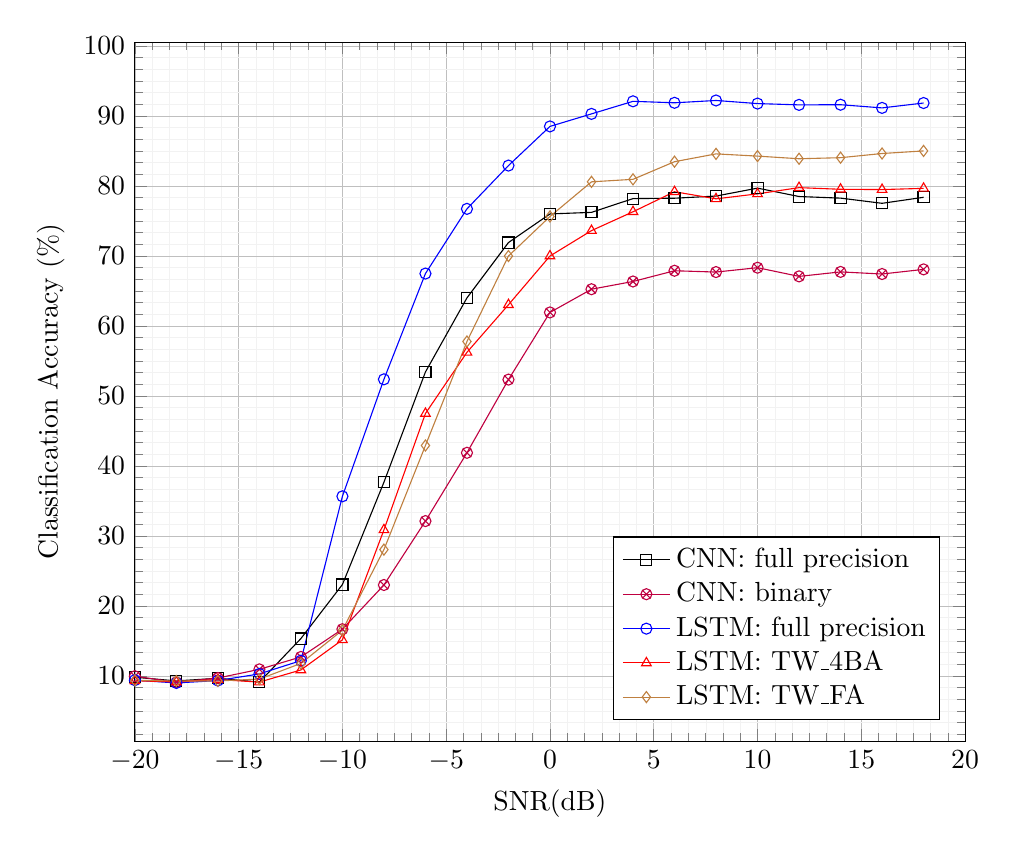
\begin{tikzpicture} \begin{axis}[legend pos=south east,
 width=\columnwidth,
 grid=both,
 ylabel=Classification Accuracy (\%),
  xlabel=SNR(dB),
 grid style={line width=.1pt, draw=gray!10},
 major grid style={line width=.2pt,draw=gray!50},
 minor tick num=5,
 xmin=-20,
 xmax=20,
 legend cell align={left},
]

\addplot[mark=square, color=black] coordinates { 
(-20, 09.807868252516011) (-18, 09.282470481380563) (-16, 09.659913169319827) (-14, 09.115341032118368) (-12, 15.332725615314494) (-10, 23.049582370712635) (-8, 37.6630534631637) (-6, 53.40909090909091) (-4, 63.99260628465804) (-2, 71.89767779390421) (0, 75.98540145985402) (2, 76.20865139949109) (4, 78.1754772393539) (6, 78.23104693140794) (8, 78.53922452660054) (10, 79.67213114754098) (12, 78.47184501176897) (14, 78.2432183059605) (16, 77.50226244343892) (18, 78.36183618361836) };
\addlegendentry{CNN: full precision}
\addplot[mark=otimes, color=purple] coordinates { 
( -20 , 9.95425434584 )  ( -18 , 9.08265213442 )  ( -16 , 9.69609261939 )  ( -14 , 10.9346806207 )  ( -12 , 12.7073837739 )  ( -10 , 16.6696285765 )  ( -8 , 22.9836487231 )  ( -6 , 32.1114369501 )  ( -4 , 41.8669131238 )  ( -2 , 52.3222060958 )  ( 0 , 61.9160583942 )  ( 2 , 65.2308251545 )  ( 4 , 66.3362701909 )  ( 6 , 67.8700361011 )  ( 8 , 67.6825969342 )  ( 10 , 68.306010929 )  ( 12 , 67.0650009053 )  ( 14 , 67.7062188596 )  ( 16 , 67.4027149321 )  ( 18 , 68.0648064806 ) };
\addlegendentry{CNN: binary}
\addplot[mark=o, color=blue] coordinates {
(-20, 09.387008234217749) (-18, 08.991825613079019) (-16, 09.334298118668596) (-14, 10.285095633345363) (-12, 12.178669097538743) (-10, 35.64954682779456) (-8,  52.36083042439831) (-6,  67.46700879765396) (-4,  76.7097966728281) (-2,  82.89187227866474) (0, 88.48540145985402) (2, 90.27626317702654) (4, 92.0704845814978) (6, 91.85920577617328) (8, 92.19116321009919) (10, 91.74863387978142) (12, 91.56255658156799) (14, 91.58516331426463) (16, 91.13122171945701) (18, 91.82718271827183)
};
\addlegendentry{LSTM: full precision}
\addplot[mark=triangle, color=red] coordinates {
(-20, 09.307868252516011) (-18, 09.132470481380563) (-16, 09.479913169319827) (-14, 09.115341032118368) (-12, 10.847725615314494)(-10,15.150416817687568) (-8, 30.853792598021251) (-6, 47.477477477477475) (-4, 56.218637992831544) (-2, 63.014450338394001) (0,  69.974508375819378) (2,  73.602656336469285) (4,  76.295479603087102) (6,  79.15686629274471) (8,  78.14148026913984) (10, 78.852849551035364) (12, 79.740828618361015) (14, 79.506573023590854) (16, 79.46428571428571) (18, 79.637277787753635)
};
\addlegendentry{LSTM: TW\_4BA}
\addplot[mark=diamond, color=brown] coordinates {
(-20, 09.368709972552608) (-18, 09.264305177111716) (-16, 09.280028943560058) (-14, 09.545290508841574) (-12, 11.777575205104832) (-10, 16.527456904211835) (-8,  28.036009553555025) (-6,  42.906891495601174) (-4,  57.7634011090573) (-2,  69.97460087082729) (0,   75.62043795620438) (2,   80.57070156306797) (4,   80.9287812041116) (6,   83.44765342960289) (8,   84.56266907123535) (10,  84.24408014571949) (12,  83.86746333514394) (14,  84.01919173279203) (16,  84.61538461538461) (18,  84.98649864986498)
};
\addlegendentry{LSTM: TW\_FA}
\end{axis}
\end{tikzpicture}
\caption{Classification accuracy of two layer quantized models on RadioML dataset.}
\label{fig_quant_acc}
\end{figure}

Most of the machine learning frameworks such as Tensorflow have started supporting quantized models for low-end processor deployment. The quantized kernels are under active development at the time of writing this paper which currently only supports a minimum quantization of 8 bit. Quantized kernels for all operations in all platforms are not available in these libraries resulting in low performance than expected. The full \ac{iq} information model classification performances on various platforms such as Nvidia GPUs, Intel and ARM processors for full precision and 8bit precision models are summarized in Table~\ref{table_perf_comp}. To avoid implementation mismatches across various models and platforms all the comparisons are done using quantization tools provided by Google's Tensorflow which is currently under active development. These tools allow to freeze and compress a trained model to a single file and then test it on various platforms easily. These values in the table are performance indicators in number of classifications per second for 128 sample length vectors. It can be noticed that the quantized models perform very bad on GPUs and Intel PCs due to lack of support. The quantized models currently provide performance very close to floating point variants on ARM processors. Quantized kernel support is improving for ARM processors due to increased demand for deploying these models on mobile devices. The aforementioned advantages of quantized models is expected to be available in the near future through these standard libraries.